\chapter{Die Funktionsweise von Self-Attention}

Transformer arbeiten mit dem zentralen Baustein Self-Attention.
Umgesetzt wird diese Self-Attention mit der \enquote{Scaled Dot-Product Attention} (vgl. \cite[S. 4]{attention}).
Self-Attention ist ein Algorithmus der letztendlich Zusammenhänge zwischen Wörtern z.B. in einem Text aufzeigt.
Wörter werden in Form von Tokens verarbeitet, die ganze Wörter oder Wortteile sein können.
Jeder Token ist einzigartig und wird zunächst nur durch eine natürliche Zahl repräsentiert.

\section{Generierung von Embeddings}

Grundlage jedes Attention-Zyklus sind Eingabe-Tokens.
Um die mathematische Vorgehensweise besser zu veranschaulichen, wird im Folgenden der Satz \enquote{Ich sitze auf der Bank} als Beispiel verarbeitet.
Dafür wird auf das Transformer-Model \enquote{BERT} (eng. Bidirectional Encoder Representations from Transformers) zurückgegriffen.
Jedes dieser Wörter ist ein eigener Token, der vor der Eingabe in den Attention-Zyklus vom Transformer übersetzt wird:
[\enquote{[CLS]}, \enquote{Ich}, \enquote{s}, \enquote{##itze}, \enquote{auf}, \enquote{der}, \enquote{Bank}, \enquote{[SEP]}].  
\enquote{[CLS]} ist ein Klassifizierungstoken, der am Anfang jeder Eingabesequenz eingefügt wird.
\enquote{[SEP]} trennt verschiedene Teile dieser Eingabesequenz (vgl. \cite[S. 221]{paass.2020}).
Diese Tokens sehen für das Model wie folgt aus: [3, 1671, 19, 3031, 115, 21, 2565, 4].
Die Herausforderung für den Transformer besteht darin, aus dem Kontext der anderen Tokens zu erkennen, ob \enquote{Bank} eine Sitzbank oder das Finanzinstitut Bank bedeutet.

Jeder Token bildet ein Schlüssel-Werte-Paar (vgl. \cite[S. 172]{paass.2020}).
Der korrespondierende Wert hinter einem Token ist ein Vektor, der die Bedeutung eines Tokens hinsichtlich mehrerer Dimensionen beschreibt.  
Diese Vektoren sind aus Trainingsdaten des Transformer-Modells entstanden.

Im ersten Schritt des Attention-Zyklus wird jeder Token in den dazugehörigen Vektor übersetzt.  
Diese Vektoren werden in der Matrix $\mathbf{X}$ gespeichert, wobei jede Zeile einen Token repräsentiert.  
Dieser Prozess wird als \textbf{Embedding} bezeichnet.  
Jeder dieser Vektoren hat gemäß der Literatur mindestens 512 Dimensionen (vgl. \cite[S. 3]{attention}).  
Es wird von einem \( d_{\text{model}} = 512 \) gesprochen.  
Es gilt: Je größer das \( d_{\text{model}} \), desto präziser kann der Transformer die Zusammenhänge zwischen Tokens erkennen.

Wenn sich Tokens im Vektorraum nahe liegen, haben sie eher Gemeinsamkeiten im Vergleich zu Tokens, die weit auseinander liegen.  
Angenommen, es gäbe nur ein \( d_{\text{model}} = 2 \) für jeden Token, könnten diese zwei Dimensionen als Koordinaten genutzt werden, um Zusammenhänge visuell als Cluster in einem Koordinatensystem darzustellen.  
Hier wären beispielsweise die Tokens \enquote{Hund} und \enquote{Katze} nah beieinander.

Für das oben genannte Beispiel nehmen verwendet das BERT-Model ein \( d_{\text{model}} = 768 \) (vgl. \cite[K. 3]{bert}).  
So ergibt sich eine Embedding-Matrix $\mathbf{X}$ mit 8 Zeilen für 8 Tokens und 768 Spalten für jeweils 768 Dimensionen, die hier der Übersicht halber gekürzt wurden:

\[
\mathbf{X} =
\begin{bmatrix}
0.7253 & 0.5980 & 0.3832 & -0.4561 & -0.4408 & \dots \\
-0.0426 & 0.5711 & 0.5014 & 0.0966 & 0.2337 & \dots \\
-0.1419 & -0.3099 & 0.6065 & -0.7789 & -1.4375 & \dots \\
0.3103 & 0.6196 & 0.5179 & -0.3268 & -1.1570 & \dots \\
0.4239 & 0.1928 & 0.5373 & -0.3288 & 0.5128 & \dots \\
0.2884 & -0.1722 & 0.5571 & -0.8964 & 0.9640 & \dots \\
0.1143 & -0.7712 & 0.7079 & -0.4984 & 0.4281 & \dots \\
0.8331 & 1.5817 & 1.6687 & -0.6492 & 0.2110 & \dots \\
\end{bmatrix}
\]

\section{Lineare Transformation in Query-, Key- und Value-Matrizen}

Die Embedding-Matrix $\mathbf{X}$ wird durch drei Gewichtungsmatrizen $\mathbf{W_Q}$, $\mathbf{W_K}$ und $\mathbf{W_V}$, die aus dem Training des Transformer-Modells stammen, in drei neue Matrizen transformiert (vgl. \cite[S. 209]{paass.2020}):

\[
\mathbf{Q} = \mathbf{X} \cdot \mathbf{W_Q}
\]
\[
\mathbf{K} = \mathbf{X} \cdot \mathbf{W_K}
\]
\[
\mathbf{V} = \mathbf{X} \cdot \mathbf{W_V}
\]

Die drei Matrizen haben im Attention-Zyklus umgangssprachlich formuliert folgende Funktionen:

\begin{itemize}
    \item \textbf{Query-Matrix (\(\mathbf{Q}\))}: Was fragt ein Token?
    \item \textbf{Key-Matrix (\(\mathbf{K}\))}: Welche Tokens im Kontext antworten am besten auf die Frage?
    \item \textbf{Value-Matrix (\(\mathbf{V}\))}: Erlernten Informationen über ein Token.
\end{itemize}

Im Beispiel sehen die jeweiligen Zeilen der Matrizen \(\mathbf{Q}\), \(\mathbf{K}\), \(\mathbf{V}\) für das Token \enquote{Bank} folgendermaßen aus:

\[
\begin{aligned}
\math{Q}_{\text{Bank}} &= [-0.13, 0.11, 0.37, 0.37, \dots], \quad 
\math{K}_{\text{Bank}} &= [0.33, 0.14, 0.20, 0.14, \dots], \quad 
\math{V}_{\text{Bank}} &= [0.44, 0.43, 0.60, 0.55, \dots]
\end{aligned}
\]


\section{Berechnung und Einbeziehung von Attention-Scores}

Um die Relevanz zwischen \(\math{Q}\) und \(\math{K}\) zu messen, wird jeweils das Skalarprodukt zwischen jedem Tokenvektor von \(\math{Q}_{\text{T}}\) und \(\math{K}_{\text{T}}\) gebildet (vgl. \cite[S. 209]{paass.2020}).  
Also im Beispiel wird unter anderem der Tokenvektor \(\math{Q}_{\text{Bank}}\) mit jedem Tokenvektor \(\math{K}_{\text{T}}\) multipliziert.

Die berechneten Attentionscores müssen noch zwei Verfahren unterlaufen.
Einmal ist das die Fokussierung und Normalisierung der Attentionscores mit der \textbf{Softmax-Funktion}.
\[
\text{Softmax}(x_i) = \frac{\exp(x_i)}{\sum_{j} \exp(x_j)}
\]

\(\math{x}\) ist der jeweilige aktuell zu betrachtende Attention-Score-Vektor.  
\(i\) ist der aktuell zu betrachtende Werteindex in diesem Vektor.  
\(j\) ist die Gesamtanzahl an Werten in \(\math{x}\).

Bei der \textbf{Fokussierung} werden höhere Attention-Score-Werte zwischen \(\mathbf{Q}\) und \(\mathbf{K}\) exponentiell bevorzugt.  
Analog dazu werden niedrigere Attention-Score-Werte exponentiell nach unten bewertet.  
Bei der zweiten Aufgabe der Softmax-Funktion, der \textbf{Normalisierung}, werden die Attention-Score-Werte pro Score-Vektor in Wahrscheinlichkeiten zwischen \(0\) und \(1\) transformiert, wobei die Summe jedes Attention-Score-Vektors immer \(1\) ist (vgl. \cite[K. II.B]{attention}).

Damit die Softmax-Funktion aber optimal funktionieren kann, müssen die Werte in den Attention-Score-Vektoren erst einmal \enquote{dimensioniert} werden.
Bei geläufigen Transformermodellen wird wie oben beschrieben, ein \( d_{\text{model}} \) von mindestens 512 verwendet.
Durch diese großen Dimensionen entehen bei der Berechnung von den Attention-Scores durch die Aufsummierung bei der Bildung des Skalarprodukte sehr große Werte.
Diese großen Werte sorgen dafür, dass die Softmax-Funktion viele Q-K-Beziehungen sehr hoch bewertet und so der Transformer nicht sich auf die tatsächlich vielversprechenden Verbindungen konzentrieren kann und so die Weiterverarbeitung ungenau wird.

Um hohe Attention-Score-Werte zu normalisieren, werden die Attention-Score-Vektor-Werte durch \( \sqrt{d_{\text{model}}} \) geteilt und so für die Softmax-Funktion in einen stabilen Bereich gebracht (vgl. \cite[S. 4]{attention}).
So kann ein Transformer auch kleine Relevanzunterschiede in der Token-Beziehung berücksichtigen.
Hier beispielsweise für das Attention-Score-Array von \enquote{Bank}:

\[
\frac{\text{Scores}_{\text{Bank}}}{\sqrt{768}} = [-1.203, -1.637, -0.721, -0.814, \dots]
\]

\[
\text{Softmax}\left(\frac{\text{Scores}_{\text{Bank}}}{\sqrt{768}}\right) = [0.088, 0.060, 0.0996, 0.0786, \dots]
\]

Damit diese nun umgewandelten Attention-Score-Wahrscheinlichkeiten in den weiteren Verarbeitungsschritten berücksichtigt werden können, werden sie mit der \( V \)-Matrix multipliziert (vgl. \cite[S. 4]{attention}). 
Das zeigt dem Modell, zu wie viel Prozent der erlernten Informationen zu einem Token im nächsten Schritt einfließen.
Insgesamt sieht das Verfahren folgendermaßen aus:

\[
\text{Attention}(Q, K, V) = \operatorname{Softmax}\left(\frac{QK^T}{\sqrt{d_{\text{model}}}}\right) V
\]

Diese Berechnung wurde auch auf das das begleitende Beispiel angewendet.
Wenn die Beziehungen zwischen den Token in einer Heatmap visualisiert werden, lässt sich so z.B. erkennen, dass das Model einen hohen Zusammenhang zwischen \enquote{s}, \enquote{#itze} und \enquote{Bank} erkannt hat (siehe \ref{fig:heatmap}). 
So kann aus dem Kontext erschlossen werden, dass es sich bei Sitzen und Bank wahrschlich um eine Sitzbank handelt und nicht um das Finanzinstitut.

\begin{figure}[ht]
	\centering
	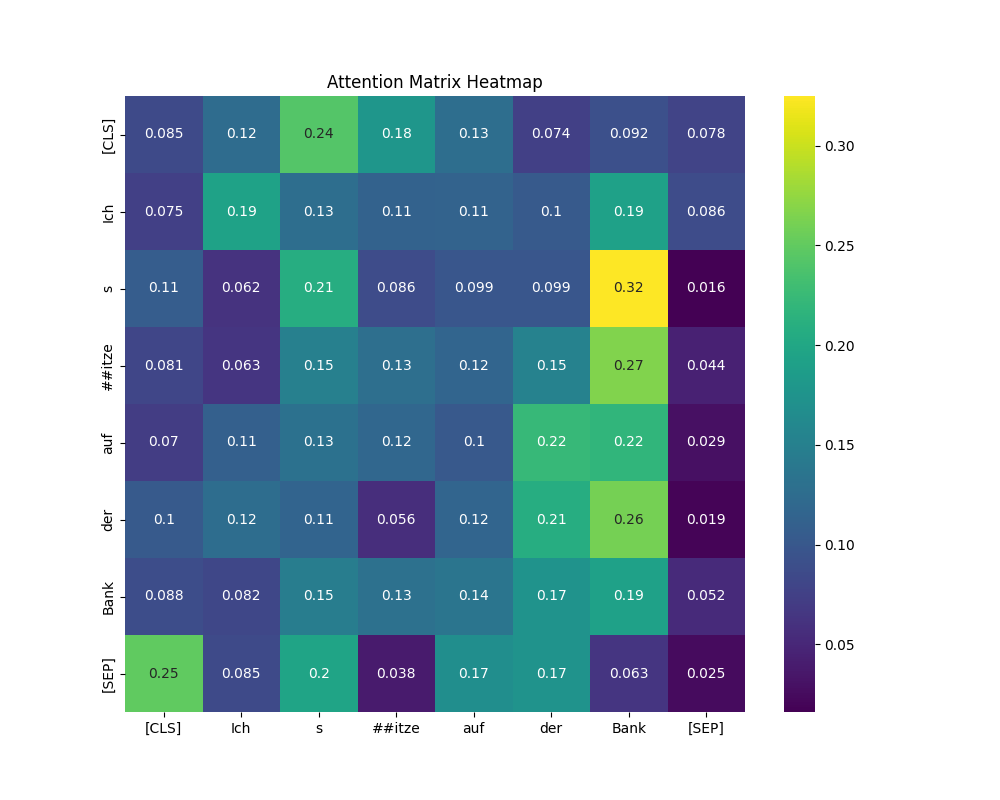
\includegraphics[width=0.8\textwidth]{Bilder/attention_matrix_heatmap.png} 
	\caption{Heatmap der gewichteten Attention Scores}
	\label{fig:heatmap}
\end{figure}

Der Vorgang hinter der \enquote{Scaled Dot-Product Attention} ist nocheinmal in der Abbildung \ref{fig:scaled-dot} zusammengefasst.

\begin{figure}[ht]
	\centering
	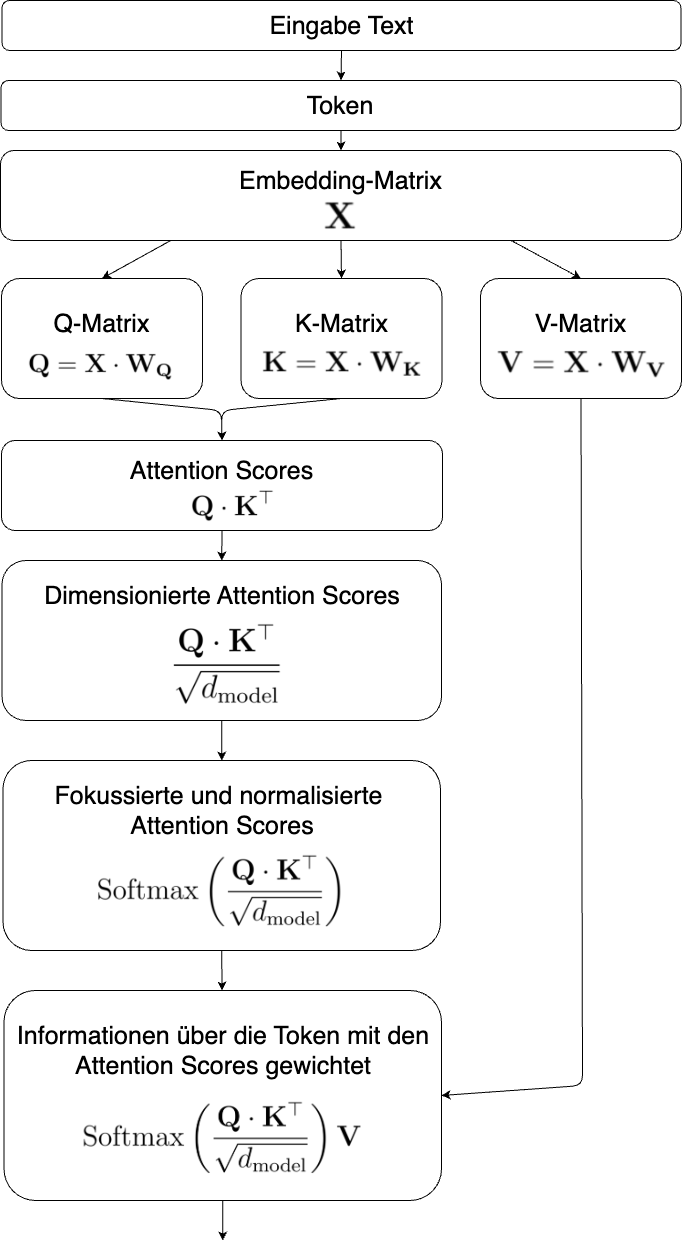
\includegraphics[width=0.6\textwidth]{Bilder/scaled-dot-attention-math.png} 
	\caption{Übersicht zur Errechnung von Attention Scores}
	\label{fig:scaled-dot}
\end{figure}